\documentclass[11pt,a4paper]{article}

\usepackage[margin=1in]{geometry}
\usepackage[T1]{fontenc}
\usepackage[utf8]{inputenc}
\usepackage{lmodern}
\usepackage{microtype}
\usepackage{amsmath, amssymb, amsfonts}
\usepackage{booktabs}
\usepackage{longtable}
\usepackage{array}
\usepackage{multirow}
\usepackage{xcolor}
\usepackage{hyperref}
\usepackage{enumitem}
\usepackage{graphicx}
\usepackage{tikz}
\usepackage{pgfplots}
\pgfplotsset{compat=1.18}
\usetikzlibrary{arrows.meta, positioning, shapes.geometric, fit, backgrounds, matrix}

\hypersetup{
  colorlinks=true,
  linkcolor=blue!60!black,
  urlcolor=blue!60!black,
  citecolor=blue!60!black,
  pdftitle={Graph-Aware Stance Detection Model Report},
  pdfauthor={OpenAI Codex}
}

\title{Graph-Aware Stance Detection for Syncialo\\
\large A Research-Oriented Technical Report on Architecture, Features, Training, and Evaluation}
\author{Technical research report}
\date{\today}

\begin{document}
\maketitle

\begin{abstract}
This document presents a research-style analysis of a graph-aware stance detection model for debate-graph relation classification. The model addresses three-way directed relation prediction between claims, where each candidate edge must be classified as \texttt{support}, \texttt{attack}, or \texttt{neutral}. The approach combines two pretrained transformer-based subsystems, namely a natural language inference model and a target-dependent stance detector, with a debate-local graph feature extractor built from TF--IDF similarity structure. These heterogeneous signals are fused into a thirteen-dimensional representation and classified with a Random Forest. This report details the mathematical structure of the features, the debate-local graph construction process, the training protocol, the benchmark methodology, and the empirical comparison against older baselines and the earlier DeBERTa + stance logistic regression-regression model. It also includes architecture figures, metric bar charts, and confusion matrix visualizations intended to make the model suitable for exposition in a research-paper context.
\end{abstract}

\section{Introduction}
The project already contained two important ingredients:
\begin{enumerate}[label=\arabic*.]
  \item strong text-pair base models for natural language inference and target-dependent stance detection, and
  \item graph-centric downstream tooling for exporting debate graphs, visualizing them, and running discourse-oriented graph algorithms.
\end{enumerate}

The graph-aware model was introduced to bridge these two parts. Instead of treating edge classification as a purely local sentence-pair problem, the model augments pairwise transformer features with per-debate structural and similarity-based graph features. In effect, the model asks not only ``Does claim \(u\) support or attack claim \(v\)?'' but also ``How are \(u\) and \(v\) positioned inside the semantic neighborhood of the debate graph?''

\section{Problem Formulation}
Each example corresponds to a directed candidate relation between two claims from the same debate:
\begin{equation}
e = (u, v, y)
\end{equation}
where:
\begin{itemize}[leftmargin=1.5em]
  \item \(u\) is the source claim,
  \item \(v\) is the target claim,
  \item \(y \in \{\texttt{support}, \texttt{attack}, \texttt{neutral}\}\).
\end{itemize}

The code uses the following text-pair convention:
\begin{itemize}[leftmargin=1.5em]
  \item \textbf{premise} \(=\) target claim text,
  \item \textbf{hypothesis} \(=\) source claim text.
\end{itemize}

This means the model predicts the relation from the current source claim to the target claim while using the target as the reference statement in both the NLI and stance components.

\section{Method}
\subsection{Notation}
\begin{center}
\begin{tabular}{ll}
\toprule
Symbol & Meaning \\
\midrule
\(u\) & source claim in a directed candidate relation \\
\(v\) & target claim in a directed candidate relation \\
\(e=(u,v,y)\) & labeled candidate edge \\
\(y\) & gold label in \(\{\texttt{support},\texttt{attack},\texttt{neutral}\}\) \\
\(\mathcal{C}=\{c_1,\dots,c_n\}\) & set of all claims in one debate \\
\(\mathbf{t}_i\) & TF--IDF vector of claim \(c_i\) \\
\(N_k(c_i)\) & retained top-\(k\) similarity-neighbor set of claim \(c_i\) \\
\(k\) & neighborhood size limit in the similarity graph \\
\(\tau\) & similarity threshold for retaining neighbors \\
\(\mathbf{x}_{\mathrm{NLI}}\) & 3-dimensional NLI logit vector \\
\(\mathbf{x}_{\mathrm{stance}}\) & 3-dimensional stance logit vector \\
\(\mathbf{x}_{\mathrm{graph}}\) & 7-dimensional graph feature vector \\
\(\mathbf{x}_{\mathrm{full}}\) & fused 13-dimensional feature vector \\
\(\hat{\mathbf{p}}(\mathbf{x})\) & predicted class probability vector \\
\(\hat{y}\) & predicted class label \\
\bottomrule
\end{tabular}
\end{center}

\subsection{Dataset and Label Construction}
\subsection{Dataset Source}
The current graph-aware benchmark uses the Syncialo raw dataset:
\begin{itemize}[leftmargin=1.5em]
  \item repository id: \texttt{DebateLabKIT/syncialo-raw}
  \item corpus: \texttt{synthetic\_corpus-001}
  \item split: \texttt{eval}
\end{itemize}

Each debate file is a node-link JSON graph. The project parses:
\begin{itemize}[leftmargin=1.5em]
  \item \texttt{nodes} to obtain claim texts,
  \item \texttt{links} to obtain gold \texttt{PRO}/\texttt{CON} relations.
\end{itemize}

\subsection{Gold Labels}
Gold labels are mapped as follows:
\begin{align*}
\texttt{PRO} &\mapsto \texttt{support} \\
\texttt{CON} &\mapsto \texttt{attack}
\end{align*}

To train a three-way classifier, the benchmark additionally samples non-edges from the same debate graph and labels them as \texttt{neutral}. The current configuration uses:
\[
\texttt{neutrals\_per\_pos} = 1.0
\]
so the intended class mixture is approximately one neutral example for every positive edge, subject to sampling availability.

\subsection{Per-Debate Processing}
All graph-aware feature construction is local to an individual debate. This is a crucial design decision:
\begin{itemize}[leftmargin=1.5em]
  \item candidate source--target pairs are formed within the same debate only,
  \item semantic neighborhoods are built only from claims within the same debate,
  \item graph features are not allowed to connect claims across debates.
\end{itemize}

However, the final classifier is trained across multiple debates to improve generalization.

\subsection{Base Transformer Components}
\subsubsection{Base NLI Model}
The NLI feature block is produced by a Hugging Face sequence classifier loaded from:
\[
\texttt{MoritzLaurer/DeBERTa-v3-large-mnli-fever-anli-ling-wanli}
\]

Its output logits are canonicalized to the three-dimensional vector:
\begin{equation}
\mathbf{x}_{\text{NLI}} = [\ell_{\text{contradiction}}, \ell_{\text{neutral}}, \ell_{\text{entailment}}]
\end{equation}

\subsubsection{Base Stance Model}
The stance feature block is produced by a target-dependent stance classifier loaded from:
\[
\texttt{krishnagarg09/stance-detection-semeval2016}
\]

It returns logits in the canonical order:
\begin{equation}
\mathbf{x}_{\text{stance}} = [\ell_{\text{against}}, \ell_{\text{none}}, \ell_{\text{favor}}]
\end{equation}

In the implementation, the tokenizer input order is:
\[
(\text{claim}, \text{target})
\]
which, under the project convention, becomes:
\[
(\text{source claim}, \text{target claim})
\]

\subsubsection{Meta Baseline}
Before the graph-aware model was added, the main learned combination layer was a multinomial logistic regression classifier over the concatenated six-dimensional transformer feature vector:
\begin{equation}
\mathbf{x}_{\text{base}} =
\left[
\mathbf{x}_{\text{NLI}} \; ; \; \mathbf{x}_{\text{stance}}
\right]
\in \mathbb{R}^{6}
\end{equation}

This remains the main non-graph baseline for comparison.

\subsection{Graph-Aware Feature Design}
\subsubsection{Motivation}
The six transformer logits are informative but fundamentally local: they encode how the source and target claims interact as a pair, but they do not encode how those claims are situated inside the rest of the debate. In structured discourse, this omission matters. Claims that are semantically central, claims that share neighborhoods, and claims that occur inside overlapping topical regions may exhibit relation patterns that are not recoverable from pairwise text alone. The graph-aware model therefore augments the local transformer evidence with seven debate-local graph features derived from a similarity graph constructed over all claims in the same debate.

\subsubsection{TF--IDF Construction}
The debate-local graph begins with a sparse lexical-semantic representation of every claim in one debate. Let a debate contain claims \(c_1,\dots,c_n\). For a vocabulary term \(t\) and document claim \(c_i\), the term frequency component is:
\begin{equation}
\mathrm{tf}(t,c_i) = \text{number of occurrences of term } t \text{ in } c_i
\end{equation}
In standard vectorized form, one often uses a normalized or sublinear version of this count, but the practical effect is the same: more salient terms in a claim receive larger local weights.

The inverse document frequency component is:
\begin{equation}
\mathrm{idf}(t,\mathcal{C}) = \log\left(\frac{1 + |\mathcal{C}|}{1 + |\{c \in \mathcal{C} : t \in c\}|}\right) + 1
\end{equation}
where \(\mathcal{C}\) is the set of claims in the current debate. The debate-local TF--IDF weight is then:
\begin{equation}
\mathrm{tfidf}(t,c_i,\mathcal{C}) = \mathrm{tf}(t,c_i)\cdot \mathrm{idf}(t,\mathcal{C})
\end{equation}

In the implementation, TF--IDF is computed \emph{per debate}, not across the entire dataset. This design choice is important. The vocabulary statistics are therefore conditioned on the current debate only:
\begin{itemize}[leftmargin=1.5em]
  \item if a term is rare within one debate, it becomes salient in that debate,
  \item if a term is common across many claims in the same debate, its discriminative value decreases.
\end{itemize}

This local fitting behavior is appropriate for graph-aware relation modeling because the objective is to recover neighborhood structure inside each debate rather than to build a global corpus-wide retrieval system.

The implementation uses:
\begin{itemize}[leftmargin=1.5em]
  \item English stop-word removal,
  \item \texttt{max\_features = 4000},
  \item a separate TF--IDF fit for every debate.
\end{itemize}

\subsubsection{Similarity Graph Construction}
Let \(\mathbf{t}_i\) denote the TF--IDF vector for claim \(c_i\). Pairwise similarity is computed via cosine similarity:
\begin{equation}
\mathrm{sim}(c_i,c_j) =
\cos(\mathbf{t}_i,\mathbf{t}_j)
=
\frac{\mathbf{t}_i^\top \mathbf{t}_j}{\|\mathbf{t}_i\|_2 \|\mathbf{t}_j\|_2}
\end{equation}

For each source claim \(c_i\), the system ranks all other claims by decreasing cosine similarity and retains only neighbors satisfying both conditions:
\begin{enumerate}[label=\arabic*.]
  \item \(\mathrm{sim}(c_i,c_j) \ge \tau\)
  \item the neighbor is among the top-\(k\) most similar claims
\end{enumerate}

For the saved benchmark:
\[
k = 8, \qquad \tau = 0.15
\]

This produces a directed local neighborhood set:
\begin{equation}
N_k(c_i) = \{c_j : c_j \text{ retained as one of the top-}k\text{ neighbors of } c_i\}
\end{equation}

\subsubsection{Formal Feature Vector}
For a directed candidate edge \((u,v)\), the graph-aware feature extractor returns:
\begin{equation}
\mathbf{x}_{\text{graph}}(u,v) =
\begin{bmatrix}
f_1(u,v) & f_2(u,v) & f_3(u,v) & f_4(u,v) & f_5(u,v) & f_6(u,v) & f_7(u,v)
\end{bmatrix}
\in \mathbb{R}^7
\end{equation}

\subsubsection{Feature 1: Cosine Similarity}
The first feature is the TF--IDF cosine similarity between the source and target claims:
\begin{equation}
f_1(u,v) = \mathrm{sim}(u,v)
\end{equation}

This feature measures lexical-semantic proximity inside the current debate. It is useful because relations such as support frequently arise between semantically close claims or paraphrastic elaborations, while very weak similarity can be a useful cue for neutrality. At the same time, attack edges can also retain moderate similarity because rebuttals often reuse the same topic words. Thus this feature is informative but not sufficient on its own, making it a good interaction feature for the downstream classifier.

\subsubsection{Feature 2: Normalized Source Degree}
Let \(N_k(u)\) be the retained similarity-neighbor set of source claim \(u\). The normalized source degree is:
\begin{equation}
f_2(u,v) = \frac{|N_k(u)|}{\max(1,k)}
\end{equation}

This quantity measures how broadly connected the source claim is in the local semantic graph. A source claim with many similarity neighbors is often topically central or semantically generic. Such claims may behave differently from highly specific claims that attach to only a few neighbors. The feature helps the model determine whether the source is structurally central, potentially affecting the prior likelihood of support, attack, or neutral relations.

\subsubsection{Feature 3: Normalized Target Degree}
Similarly, the normalized target degree is:
\begin{equation}
f_3(u,v) = \frac{|N_k(v)|}{\max(1,k)}
\end{equation}

This feature measures how broadly connected the target claim is inside the debate-local similarity graph. A highly connected target may represent a central motion, a common theme, or a semantically broad claim that attracts many related statements. Such central targets often participate in relation patterns that differ from those of isolated targets. Including both source and target degree terms allows the model to distinguish local relation types conditioned on the structural status of both endpoints.

\subsubsection{Feature 4: Target-in-Source Neighbors}
This binary indicator tests whether the target appears in the source neighborhood:
\begin{equation}
f_4(u,v) =
\mathbf{1}[v \in N_k(u)]
\end{equation}
where \(\mathbf{1}[\cdot]\) is the indicator function.

Intuitively, this feature captures whether the source claim directly regards the target claim as one of its most similar semantic anchors. This is stronger than raw cosine similarity because it introduces a thresholded, rank-aware notion of neighborhood membership. A candidate edge whose target is explicitly retained in the source neighborhood is more likely to correspond to a meaningful discourse relation than a pair that merely has a moderate similarity score.

\subsubsection{Feature 5: Source-in-Target Neighbors}
The reciprocal membership feature is:
\begin{equation}
f_5(u,v) =
\mathbf{1}[u \in N_k(v)]
\end{equation}

This is not redundant with \(f_4\) because the retained similarity graph is directed: \(v\) can be among the top-\(k\) neighbors of \(u\) without the reverse being true. This asymmetry matters because one claim can be semantically specific relative to another. The model can therefore exploit whether the similarity relationship is one-sided or mutual.

\subsubsection{Feature 6: Neighbor-Set Jaccard Overlap}
The overlap between the similarity neighborhoods of the source and target is measured with Jaccard similarity:
\begin{equation}
f_6(u,v)
=
\mathrm{Jaccard}(N_k(u), N_k(v))
=
\frac{|N_k(u)\cap N_k(v)|}{|N_k(u)\cup N_k(v)|}
\end{equation}
with the convention that the value is \(0\) when the union is empty.

This feature measures whether the two claims live in the same local semantic region of the debate. Even if \(u\) and \(v\) are not direct nearest neighbors of one another, they may still share many neighbors. Such shared-neighborhood evidence can indicate common topical framing, parallel subarguments, or participation in the same semantic cluster. This is particularly valuable for discourse graphs where indirect neighborhood structure often matters as much as direct pair similarity.

\subsubsection{Feature 7: Token-Level Jaccard Overlap}
The final graph feature is a token-level Jaccard overlap. Let \(T(u)\) and \(T(v)\) denote the lowercase whitespace-token sets of the source and target claims. Then:
\begin{equation}
f_7(u,v)
=
\mathrm{Jaccard}(T(u), T(v))
=
\frac{|T(u)\cap T(v)|}{|T(u)\cup T(v)|}
\end{equation}

This feature provides a simpler lexical overlap signal than full TF--IDF cosine similarity. It is useful because some relation cues come from literal lexical reuse, especially when one claim explicitly echoes or reframes another. It also offers robustness when TF--IDF weighting downweights common but discourse-relevant terms.

\subsubsection{Relationship Between Jaccard Similarity and Jaccard Overlap}
In this report, the terms \emph{Jaccard similarity} and \emph{Jaccard overlap} refer to the same set-based quantity:
\begin{equation}
\mathrm{Jaccard}(A,B)=\frac{|A\cap B|}{|A\cup B|}
\end{equation}
The distinction is interpretive rather than mathematical:
\begin{itemize}[leftmargin=1.5em]
  \item for \(N_k(u)\) and \(N_k(v)\), it is a \emph{neighbor-set overlap},
  \item for \(T(u)\) and \(T(v)\), it is a \emph{token-set overlap}.
\end{itemize}

\subsubsection{Final Input Representation}
The graph-aware classifier uses:
\begin{equation}
\mathbf{x}_{\text{full}} =
\left[
\mathbf{x}_{\text{NLI}} \; ; \; \mathbf{x}_{\text{stance}} \; ; \; \mathbf{x}_{\text{graph}}
\right]
\in \mathbb{R}^{13}
\end{equation}
where:
\[
\mathbf{x}_{\text{NLI}} \in \mathbb{R}^{3}, \qquad
\mathbf{x}_{\text{stance}} \in \mathbb{R}^{3}, \qquad
\mathbf{x}_{\text{graph}} \in \mathbb{R}^{7}
\]

\section{Experimental Setup}
The quantitative results reported in this document are based on a saved benchmark run with the following configuration.

\subsection{Configuration}
\begin{center}
\begin{tabular}{ll}
\toprule
Setting & Value \\
\midrule
Corpus & \texttt{synthetic\_corpus-001} \\
Split & \texttt{eval} \\
Max debates & \(8\) \\
Small mode & \texttt{true} \\
Test size & \(0.25\) \\
Seed & \(0\) \\
NLI model & \texttt{MoritzLaurer/DeBERTa-v3-large-mnli-fever-anli-ling-wanli} \\
Stance model & \texttt{krishnagarg09/stance-detection-semeval2016} \\
Similarity top-\(k\) & \(8\) \\
Similarity threshold & \(0.15\) \\
\bottomrule
\end{tabular}
\end{center}

\subsection{Train/Test Debate Split}
\textbf{Train debates}:
\begin{itemize}[leftmargin=1.5em]
  \item \texttt{node\_link\_data-debate-eval-0013}
  \item \texttt{node\_link\_data-debate-eval-0029}
  \item \texttt{node\_link\_data-debate-eval-0044}
  \item \texttt{node\_link\_data-debate-eval-0015}
  \item \texttt{node\_link\_data-debate-eval-0028}
  \item \texttt{node\_link\_data-debate-eval-0001}
\end{itemize}

\textbf{Test debates}:
\begin{itemize}[leftmargin=1.5em]
  \item \texttt{node\_link\_data-debate-eval-0037}
  \item \texttt{node\_link\_data-debate-eval-0002}
\end{itemize}

\subsection{Example Counts}
\begin{center}
\begin{tabular}{lr}
\toprule
Set & Example count \\
\midrule
Training examples & 7224 \\
Test examples & 2664 \\
\bottomrule
\end{tabular}
\end{center}

\subsection{Class Distribution}
\begin{center}
\begin{tabular}{lrrrr}
\toprule
Split & Support & Attack & Neutral & Total \\
\midrule
Train & 1806 & 1806 & 3612 & 7224 \\
Test & 666 & 666 & 1332 & 2664 \\
Overall & 2472 & 2472 & 4944 & 9888 \\
\bottomrule
\end{tabular}
\end{center}

\subsection{Training Protocol}
The benchmark uses the following training procedure:
\begin{enumerate}[label=\arabic*.]
  \item load debates and construct candidate support, attack, and neutral examples,
  \item split debates at the debate level rather than the row level,
  \item compute base transformer features for every example,
  \item compute graph features independently inside each debate,
  \item fit the final classifier on the concatenated training representation,
  \item evaluate on held-out debates only.
\end{enumerate}

\section{Architecture Diagram}
\begin{figure}[htbp]
\centering
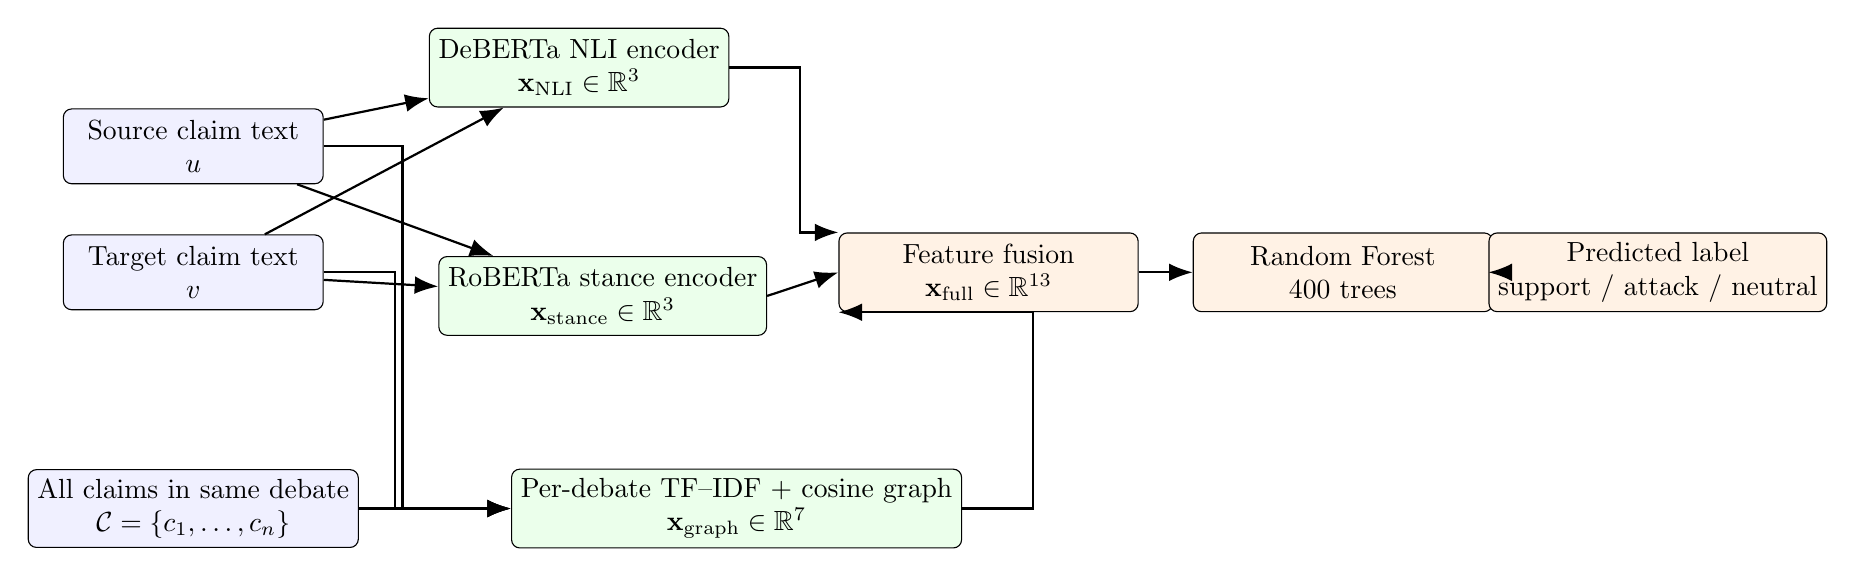
\begin{tikzpicture}[
  proc/.style={draw, rounded corners=3pt, minimum width=3.3cm, minimum height=0.95cm, align=center, fill=blue!6},
  feat/.style={draw, rounded corners=3pt, minimum width=3.6cm, minimum height=1.0cm, align=center, fill=green!8},
  cls/.style={draw, rounded corners=3pt, minimum width=3.8cm, minimum height=1.0cm, align=center, fill=orange!10},
  arrow/.style={-{Latex[length=3mm]}, thick}
]

\node[proc] (source) at (0,2.3) {Source claim text\\\(u\)};
\node[proc] (target) at (0,0.7) {Target claim text\\\(v\)};
\node[proc] (debate) at (0,-2.3) {All claims in same debate\\\(\mathcal{C}=\{c_1,\dots,c_n\}\)};

\node[feat] (nli) at (4.9,3.3) {DeBERTa NLI encoder\\\(\mathbf{x}_{\mathrm{NLI}}\in\mathbb{R}^3\)};
\node[feat] (stance) at (5.2,0.4) {RoBERTa stance encoder\\\(\mathbf{x}_{\mathrm{stance}}\in\mathbb{R}^3\)};
\node[feat] (tfidf) at (6.9,-2.3) {Per-debate TF--IDF + cosine graph\\\(\mathbf{x}_{\mathrm{graph}}\in\mathbb{R}^7\)};

\node[cls] (concat) at (10.1,0.7) {Feature fusion\\\(\mathbf{x}_{\mathrm{full}}\in\mathbb{R}^{13}\)};
\node[cls] (forest) at (14.6,0.7) {Random Forest\\400 trees};
\node[cls] (soft) at (18.6,0.7) {Predicted label\\support / attack / neutral};

\draw[arrow] (source) -- (nli);
\draw[arrow] (target) -- (nli);
\draw[arrow] (source) -- (stance);
\draw[arrow] (target) -- (stance);
\draw[arrow] (debate) -- (tfidf);
\draw[arrow] (source.east) -- ++(1.0,0) |- (tfidf.west);
\draw[arrow] (target.east) -- ++(0.9,0) |- (tfidf.west);

\draw[arrow] (nli.east) -- ++(0.9,0) |- (concat.north west);
\draw[arrow] (stance.east) -- (concat.west);
\draw[arrow] (tfidf.east) -- ++(0.9,0) |- (concat.south west);
\draw[arrow] (concat) -- (forest);
\draw[arrow] (forest) -- (soft);
\end{tikzpicture}
\caption{Revised architecture of the graph-aware stance model. The model fuses pairwise transformer evidence with debate-local graph-context features before nonlinear classification.}
\end{figure}

\subsection{Classifier Choice}
The graph-aware model uses a Random Forest classifier:
\begin{itemize}[leftmargin=1.5em]
  \item \texttt{n\_estimators = 400}
  \item \texttt{random\_state = 0}
  \item \texttt{n\_jobs = -1}
  \item \texttt{class\_weight = "balanced\_subsample"}
  \item \texttt{min\_samples\_leaf = 2}
\end{itemize}

This is a deliberate contrast to the meta baseline, which uses linear multinomial logistic regression. The rationale is straightforward:
\begin{itemize}[leftmargin=1.5em]
  \item the six transformer logits are approximately linearly useful,
  \item the graph features introduce threshold-like and interaction-heavy signals,
  \item Random Forests can model nonlinear interactions between lexical similarity, local degree patterns, and transformer confidence without requiring explicit manual feature crosses.
\end{itemize}

\subsubsection{Decision Function of the Random Forest}
Let the forest contain \(M\) decision trees, with \(M=400\) in the current implementation. For an input feature vector \(\mathbf{x}_{\text{full}}\), each tree \(T_m\) outputs a class probability distribution over the three labels:
\[
T_m(\mathbf{x}_{\text{full}}) \in [0,1]^3
\]

The forest prediction is the average probability vector:
\[
\hat{\mathbf{p}}(\mathbf{x}_{\text{full}})
=
\frac{1}{M}\sum_{m=1}^{M} T_m(\mathbf{x}_{\text{full}})
\]

The final class prediction is:
\[
\hat{y}
=
\arg\max_{c \in \{\texttt{support}, \texttt{attack}, \texttt{neutral}\}}
\hat{p}_c(\mathbf{x}_{\text{full}})
\]

This form is especially appropriate for the current feature space because it allows thresholding and feature interactions to emerge from the tree splits. For example, the model can learn that a moderate entailment logit is useful only when the target is also among the source's semantic neighbors, or that a high token overlap should be interpreted differently depending on neighborhood asymmetry.

\subsection{Detailed Training Procedure}
\subsubsection{Step 1: Debate Sampling}
The benchmark first loads debates from Syncialo and shuffles them with a fixed seed. In the saved experiment, the first eight debates from the shuffled order were used because small mode was active.

\subsubsection{Step 2: Debate-Level Split}
The system then splits at the debate level, not the row level. This is important because it prevents leakage from one debate into both train and test.

\subsubsection{Step 3: Pair and Neutral Construction}
For each debate:
\begin{enumerate}[label=\arabic*.]
  \item include all gold support/attack edges,
  \item sample non-edge pairs from the same debate,
  \item label sampled non-edges as neutral,
  \item convert each pair into \((\text{premise}, \text{hypothesis}, \text{label})\).
\end{enumerate}

\subsubsection{Step 4: Base Transformer Featurization}
For each example, the system computes:
\[
\mathbf{x}_{\text{base}} =
[\ell_{\text{contradiction}}, \ell_{\text{neutral}}, \ell_{\text{entailment}},
\ell_{\text{against}}, \ell_{\text{none}}, \ell_{\text{favor}}]
\]

\subsubsection{Step 5: Graph Feature Construction}
Graph features are constructed separately for each debate using the TF--IDF similarity graph. The resulting arrays are aligned with the same training and test examples.

\subsubsection{Step 6: Model Training}
The graph-aware classifier is trained on:
\[
\mathbf{X}_{\text{train}} =
\left[
\mathbf{X}_{\text{train,base}} \; ; \; \mathbf{X}_{\text{train,graph}}
\right]
\]

\subsubsection{Step 7: Evaluation}
At test time, the system concatenates the test base features and test graph features and predicts one of the three labels.

\section{Baselines Used for Comparison}
The benchmark compares four systems.

\subsection{ DeBERTa Rule/Decision Baseline}
This baseline uses the NLI model outputs directly and then maps them into relation decisions using an older rule-based decision layer. The system therefore has a two-stage structure: a transformer encoder produces contradiction, neutral, and entailment evidence, and a hand-designed decision rule converts those outputs into one of the three discourse labels.

\begin{figure}[htbp]
\centering
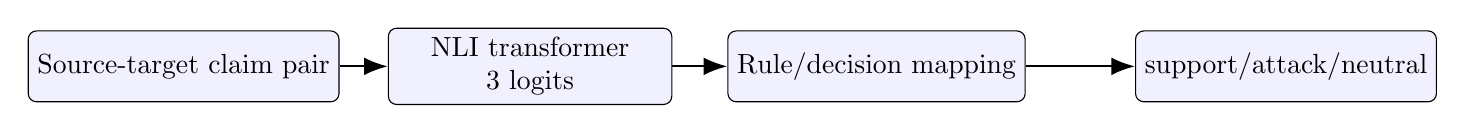
\begin{tikzpicture}[
  b/.style={draw, rounded corners=3pt, minimum width=3.6cm, minimum height=0.9cm, align=center, fill=blue!6},
  arrow/.style={-{Latex[length=3mm]}, thick}
]
\node[b] (pair) at (0,0) {Source-target claim pair};
\node[b] (nli) at (4.4,0) {NLI transformer\\3 logits};
\node[b] (rule) at (8.8,0) {Rule/decision mapping};
\node[b] (out) at (14.0,0) {support/attack/neutral};
\draw[arrow] (pair) -- (nli);
\draw[arrow] (nli) -- (rule);
\draw[arrow] (rule) -- (out);
\end{tikzpicture}
\caption{Architecture of the  DeBERTa rule/decision baseline.}
\end{figure}

\subsection{ Stance Baseline}
This baseline predicts the discourse label from the stance model alone. The target-dependent stance classifier produces logits corresponding to against, none, and favor, and these outputs are directly converted into the final stance-relation decision without any graph features or NLI evidence.

\begin{figure}[htbp]
\centering
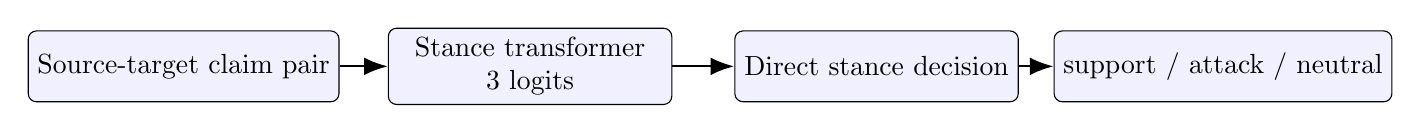
\begin{tikzpicture}[
  b/.style={draw, rounded corners=3pt, minimum width=3.6cm, minimum height=0.9cm, align=center, fill=blue!6},
  arrow/.style={-{Latex[length=3mm]}, thick}
]
\node[b] (pair) at (0,0) {Source-target claim pair};
\node[b] (stance) at (4.4,0) {Stance transformer\\3 logits};
\node[b] (decide) at (8.8,0) {Direct stance decision};
\node[b] (out) at (13.2,0) {support / attack / neutral};
\draw[arrow] (pair) -- (stance);
\draw[arrow] (stance) -- (decide);
\draw[arrow] (decide) -- (out);
\end{tikzpicture}
\caption{Architecture of the  stance-only baseline.}
\end{figure}

\subsection{DeBERTa + stance logistic regression Regression Baseline}
This is the stronger non-graph baseline. It concatenates the three NLI logits and the three stance logits into a six-dimensional vector and then fits a multinomial logistic regression classifier over that fused representation.

\begin{figure}[htbp]
\centering
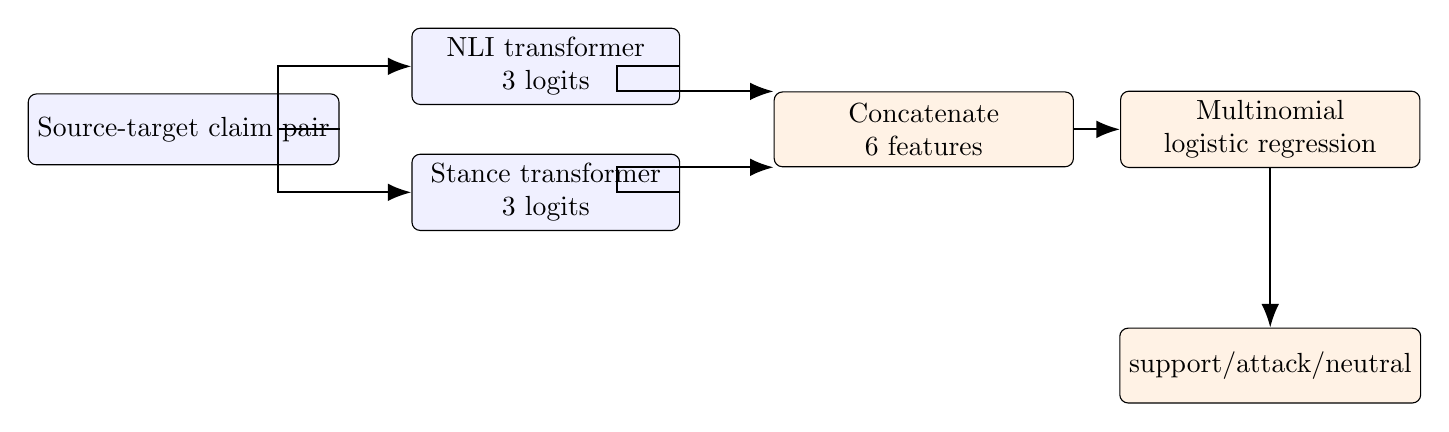
\begin{tikzpicture}[
  b/.style={draw, rounded corners=3pt, minimum width=3.4cm, minimum height=0.9cm, align=center, fill=blue!6},
  c/.style={draw, rounded corners=3pt, minimum width=3.8cm, minimum height=0.95cm, align=center, fill=orange!10},
  arrow/.style={-{Latex[length=3mm]}, thick}
]
\node[b] (pair) at (0,1.0) {Source-target claim pair};
\node[b] (nli) at (4.6,1.8) {NLI transformer\\3 logits};
\node[b] (stance) at (4.6,0.2) {Stance transformer\\3 logits};
\node[c] (concat) at (9.4,1.0) {Concatenate\\6 features};
\node[c] (lr) at (13.8,1.0) {Multinomial\\logistic regression};
\node[c] (out) at (13.8,-2.) {support/attack/neutral};
\draw[arrow] (pair) -- ++(1.2,0) |- (nli.west);
\draw[arrow] (pair) -- ++(1.2,0) |- (stance.west);
\draw[arrow] (nli) -- ++(0.9,0) |- (concat.north west);
\draw[arrow] (stance) -- ++(0.9,0) |- (concat.south west);
\draw[arrow] (concat) -- (lr);
\draw[arrow] (lr) -- (out);
\end{tikzpicture}
\caption{Architecture of the DeBERTa + stance logistic regression-regression baseline.}
\end{figure}

\subsection{Graph-Aware Model}
This is the proposed model. It uses the same six transformer features as the meta baseline, but augments them with seven debate-local graph features and swaps the linear meta-classifier for a Random Forest.

\section{Results}
\subsection{Overall Metrics}
\begin{center}
\begin{tabular}{lccc}
\toprule
Model & Accuracy & Macro-F1 & Weighted-F1 \\
\midrule
 DeBERTa baseline & 0.5601 & 0.3907 & 0.4658 \\
 stance model(semeval2017) baseline & 0.3517 & 0.3104 & 0.3349 \\
DeBERTa + stance logistic regression regression & 0.6513 & 0.6557 & 0.6477 \\
\textbf{Graph-aware model} & \textbf{0.8818} & \textbf{0.8665} & \textbf{0.8811} \\
\bottomrule
\end{tabular}
\end{center}

\subsection{Metric Comparison Bar Charts}
\begin{figure}[htbp]
\centering
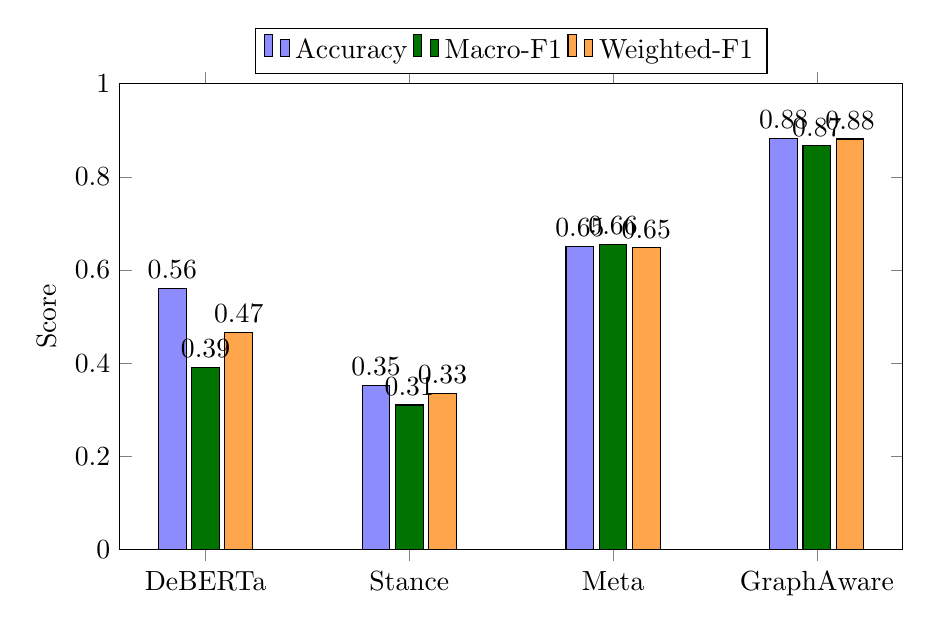
\begin{tikzpicture}
\begin{axis}[
    ybar,
    bar width=10pt,
    width=0.95\textwidth,
    height=7.5cm,
    ymin=0,
    ymax=1.0,
    ylabel={Score},
    symbolic x coords={DeBERTa,Stance,Meta,GraphAware},
    xtick=data,
    legend style={at={(0.5,1.02)}, anchor=south, legend columns=3},
    nodes near coords,
    nodes near coords align={vertical},
    enlarge x limits=0.14
]
\addplot[fill=blue!45] coordinates {
  (DeBERTa,0.5601)
  (Stance,0.3517)
  (Meta,0.6513)
  (GraphAware,0.8818)
};
\addplot[fill=green!45!black] coordinates {
  (DeBERTa,0.3907)
  (Stance,0.3104)
  (Meta,0.6557)
  (GraphAware,0.8665)
};
\addplot[fill=orange!70] coordinates {
  (DeBERTa,0.4658)
  (Stance,0.3349)
  (Meta,0.6477)
  (GraphAware,0.8811)
};
\legend{Accuracy, Macro-F1, Weighted-F1}
\end{axis}
\end{tikzpicture}
\caption{Comparison of the four evaluated models across the three primary aggregate metrics.}
\end{figure}

\subsection{Per-Class Scores}
\begin{center}
\begin{tabular}{llccc}
\toprule
Model & Class & Precision & Recall & F1 \\
\midrule
\multirow{3}{*}{ DeBERTa}
  & Support & 0.8182 & 0.1081 & 0.1910 \\
  & Attack  & \textbf{0.8722} & 0.1742 & 0.2904 \\
  & Neutral & 0.5338 & \textbf{0.9790} & 0.6909 \\
\midrule
\multirow{3}{*}{ stance}
  & Support & 0.2607 & 0.7162 & 0.3822 \\
  & Attack  & 0.2844 & 0.0931 & 0.1403 \\
  & Neutral & 0.6461 & 0.2988 & 0.4086 \\
\midrule
\multirow{3}{*}{DeBERTa + stance logistic regression}
  & Support & 0.5726 & 0.7102 & 0.6340 \\
  & Attack  & 0.6257 & 0.8183 & 0.7092 \\
  & Neutral & 0.7415 & 0.5383 & 0.6237 \\
\midrule
\multirow{3}{*}{\textbf{Graph-aware}}
  & Support & \textbf{0.8485} & \textbf{0.8243} & \textbf{0.8363} \\
  & Attack  & 0.8525 & \textbf{0.8243} & \textbf{0.8382} \\
  & Neutral & \textbf{0.9111} & 0.9392 & \textbf{0.9250} \\
\bottomrule
\end{tabular}
\end{center}

\subsection{Confusion Matrices}
Using label order \([\texttt{support}, \texttt{attack}, \texttt{neutral}]\):

\paragraph{ DeBERTa baseline}
\[
\begin{bmatrix}
72 & 2 & 592 \\
3 & 116 & 547 \\
13 & 15 & 1304
\end{bmatrix}
\]

\paragraph{ stance baseline}
\[
\begin{bmatrix}
477 & 74 & 115 \\
501 & 62 & 103 \\
852 & 82 & 398
\end{bmatrix}
\]

\paragraph{DeBERTa + stance logistic regression baseline}
\[
\begin{bmatrix}
473 & 39 & 154 \\
25 & 545 & 96 \\
328 & 287 & 717
\end{bmatrix}
\]

\paragraph{Graph-aware model}
\[
\begin{bmatrix}
549 & 56 & 61 \\
56 & 549 & 61 \\
42 & 39 & 1251
\end{bmatrix}
\]

\subsection{Confusion Matrix Figures}
\begin{figure}[htbp]
\centering
\begin{minipage}{0.48\textwidth}
\centering
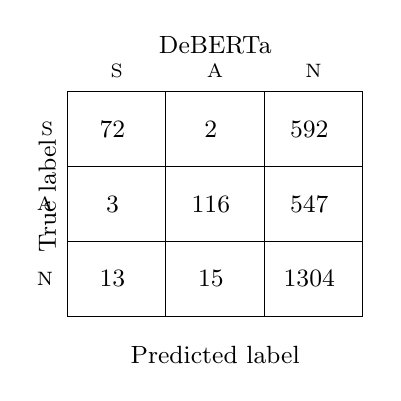
\begin{tikzpicture}[scale=0.68]
\matrix[matrix of nodes,
nodes={draw, minimum width=1.25cm, minimum height=0.95cm, align=center, font=\small},
row sep=-\pgflinewidth, column sep=-\pgflinewidth] (m) {
72 & 2 & 592 \\
3 & 116 & 547 \\
13 & 15 & 1304 \\
};
\node[above=0.35cm of m-1-2] {\small  DeBERTa};
\node[left=0.25cm of m-1-1, rotate=90] {\small True label};
\node[below=0.25cm of m-3-2] {\small Predicted label};
\node[above=0.05cm of m-1-1] {\scriptsize S};
\node[above=0.05cm of m-1-2] {\scriptsize A};
\node[above=0.05cm of m-1-3] {\scriptsize N};
\node[left=0.05cm of m-1-1] {\scriptsize S};
\node[left=0.05cm of m-2-1] {\scriptsize A};
\node[left=0.05cm of m-3-1] {\scriptsize N};
\end{tikzpicture}
\end{minipage}
\hfill
\begin{minipage}{0.48\textwidth}
\centering
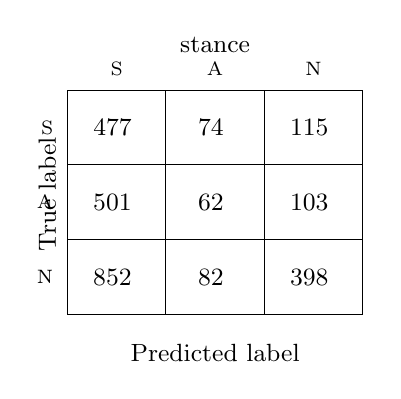
\begin{tikzpicture}[scale=0.68]
\matrix[matrix of nodes,
nodes={draw, minimum width=1.25cm, minimum height=0.95cm, align=center, font=\small},
row sep=-\pgflinewidth, column sep=-\pgflinewidth] (m) {
477 & 74 & 115 \\
501 & 62 & 103 \\
852 & 82 & 398 \\
};
\node[above=0.35cm of m-1-2] {\small  stance};
\node[left=0.25cm of m-1-1, rotate=90] {\small True label};
\node[below=0.25cm of m-3-2] {\small Predicted label};
\node[above=0.05cm of m-1-1] {\scriptsize S};
\node[above=0.05cm of m-1-2] {\scriptsize A};
\node[above=0.05cm of m-1-3] {\scriptsize N};
\node[left=0.05cm of m-1-1] {\scriptsize S};
\node[left=0.05cm of m-2-1] {\scriptsize A};
\node[left=0.05cm of m-3-1] {\scriptsize N};
\end{tikzpicture}
\end{minipage}

\vspace{0.6cm}

\begin{minipage}{0.48\textwidth}
\centering
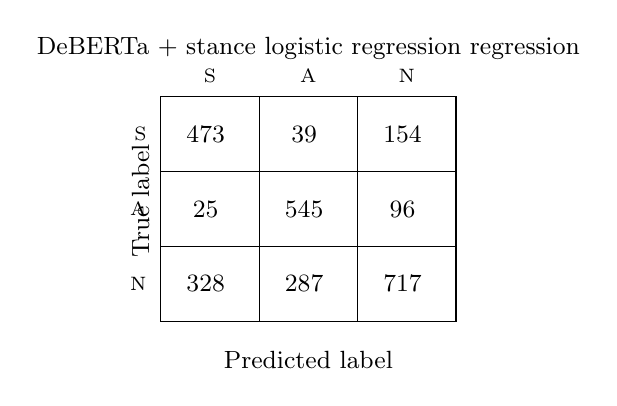
\begin{tikzpicture}[scale=0.68]
\matrix[matrix of nodes,
nodes={draw, minimum width=1.25cm, minimum height=0.95cm, align=center, font=\small},
row sep=-\pgflinewidth, column sep=-\pgflinewidth] (m) {
473 & 39 & 154 \\
25 & 545 & 96 \\
328 & 287 & 717 \\
};
\node[above=0.35cm of m-1-2] {\small DeBERTa + stance logistic regression regression};
\node[left=0.25cm of m-1-1, rotate=90] {\small True label};
\node[below=0.25cm of m-3-2] {\small Predicted label};
\node[above=0.05cm of m-1-1] {\scriptsize S};
\node[above=0.05cm of m-1-2] {\scriptsize A};
\node[above=0.05cm of m-1-3] {\scriptsize N};
\node[left=0.05cm of m-1-1] {\scriptsize S};
\node[left=0.05cm of m-2-1] {\scriptsize A};
\node[left=0.05cm of m-3-1] {\scriptsize N};
\end{tikzpicture}
\end{minipage}
\hfill
\begin{minipage}{0.48\textwidth}
\centering
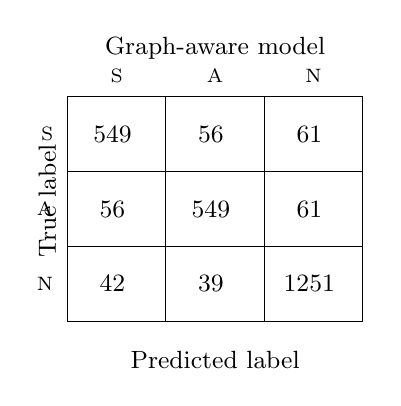
\begin{tikzpicture}[scale=0.68]
\matrix[matrix of nodes,
nodes={draw, minimum width=1.25cm, minimum height=0.95cm, align=center, font=\small},
row sep=-\pgflinewidth, column sep=-\pgflinewidth] (m) {
549 & 56 & 61 \\
56 & 549 & 61 \\
42 & 39 & 1251 \\
};
\node[above=0.35cm of m-1-2] {\small Graph-aware model};
\node[left=0.25cm of m-1-1, rotate=90] {\small True label};
\node[below=0.25cm of m-3-2] {\small Predicted label};
\node[above=0.05cm of m-1-1] {\scriptsize S};
\node[above=0.05cm of m-1-2] {\scriptsize A};
\node[above=0.05cm of m-1-3] {\scriptsize N};
\node[left=0.05cm of m-1-1] {\scriptsize S};
\node[left=0.05cm of m-2-1] {\scriptsize A};
\node[left=0.05cm of m-3-1] {\scriptsize N};
\end{tikzpicture}
\end{minipage}
\caption{Confusion matrices for all four models. Labels use the order S = support, A = attack, N = neutral.}
\end{figure}

\section{Interpretation of Results}
\subsection{Why the Graph-Aware Model Helps}
The results suggest that the graph-aware model does not merely add noise or redundant features. Instead, it substantially improves both balanced performance and absolute accuracy. There are several likely reasons.

\begin{enumerate}[label=\arabic*.]
  \item \textbf{Debate-local context reduces ambiguity.} Two claims with uncertain pairwise transformer evidence may still be easy to classify if they are very close in the local semantic neighborhood structure.
  \item \textbf{The graph features help separate neutral edges.} The graph-aware model shows a large gain on the neutral class, which is often where pure pairwise systems are unstable.
  \item \textbf{Nonlinear interactions matter.} The Random Forest can learn interactions such as:
  \begin{itemize}[leftmargin=1.5em]
    \item high semantic similarity plus strong entailment-like NLI signal,
    \item asymmetric neighborhood membership plus attack-biased stance logits,
    \item strong local overlap but weak direct textual polarity.
  \end{itemize}
  \item \textbf{The improvements are broad, not class-specific.} The graph-aware model improves support, attack, and neutral simultaneously.
\end{enumerate}

\subsection{Comparison to the  Models}
The older direct baselines show a typical pattern:
\begin{itemize}[leftmargin=1.5em]
  \item the NLI-only path overpredicts neutral,
  \item the stance-only path is unstable across classes,
  \item the DeBERTa + stance logistic regression model already gives a large boost by combining the two transformer sources,
  \item the graph-aware model adds another large jump by injecting debate-local structure.
\end{itemize}

\subsection{Comparison to the DeBERTa + stance logistic regression Baseline}
The graph-aware model improves over the meta baseline by:
\begin{align*}
\Delta \text{Accuracy} &= 0.8818 - 0.6513 \approx 0.2305 \\
\Delta \text{Macro-F1} &= 0.8665 - 0.6557 \approx 0.2108
\end{align*}

This is a very large improvement. It strongly indicates that, at least on the saved benchmark split, graph-aware local context is highly informative.

\section{Limitations and Caveats}
\subsection{The Current Benchmark Is Small}
The saved quantitative results come from the small benchmark configuration:
\begin{itemize}[leftmargin=1.5em]
  \item only eight debates,
  \item six train debates,
  \item two test debates.
\end{itemize}

These results are promising, but they should not be treated as the final word on generalization. A larger benchmark should be run before making strong performance claims.

\subsection{The Similarity Graph Is Lexical, Not Neural}
The graph-aware features are built from TF--IDF similarity, not learned graph embeddings or Graph Neural Networks. This has two implications:
\begin{itemize}[leftmargin=1.5em]
  \item it is simple, fast, and interpretable,
  \item it may miss deeper semantic relations that lexical overlap cannot capture.
\end{itemize}

\subsection{The Model Is Graph-Aware, Not a Full GNN}
Despite the name, the current model is not a message-passing neural graph model. It is better described as:
\begin{quote}
a stacked transformer-plus-graph-feature classifier.
\end{quote}

This is still valuable, but conceptually it is a feature-augmented tabular model rather than a deep graph network.

\subsection{Neutral Sampling Matters}
Neutral labels are generated by non-edge sampling. Performance on the neutral class is therefore influenced by the sampling strategy and may change if harder negatives are introduced.

\subsection{Experimental Configuration Dependence}
Different runs can use different subsets of debates, different sampling seeds, and different feature-cache states. Consequently, trained graph-aware models should be compared only when the underlying experimental configuration is controlled.

\section{Next Steps}
The current graph-aware model is a strong intermediate design. The next meaningful upgrades would be:
\begin{enumerate}[label=\arabic*.]
  \item run the benchmark on many more debates and multiple seeds,
  \item add hard-negative mining rather than purely random non-edge sampling,
  \item compute feature importance for the Random Forest,
  \item compare TF--IDF graph features with embedding-based nearest-neighbor graph features,
  \item test gradient boosting or calibrated tree ensembles,
  \item move toward iterative graph refinement or a true GNN if larger-scale training becomes feasible.
\end{enumerate}

\section{Conclusion}
The graph-aware model studied here is a practical and effective extension of a transformer-based stance pipeline. It combines:
\begin{itemize}[leftmargin=1.5em]
  \item transformer-based textual reasoning,
  \item debate-local graph context,
  \item a nonlinear final classifier.
\end{itemize}

On the current saved Syncialo benchmark split, it substantially outperforms:
\begin{itemize}[leftmargin=1.5em]
  \item the older direct NLI baseline,
  \item the older direct stance baseline,
  \item the DeBERTa + stance logistic regression-regression baseline.
\end{itemize}

Its main contribution is not merely stronger classification accuracy, but a tighter alignment between stance prediction and discourse graph structure. That makes it especially suitable for a system whose downstream goals include graph export, visualization, clustering, centrality analysis, and broader discourse interpretation.

\end{document}
